% !TEX root =  master.tex
\chapter{Speichern der Daten (Moritz Werr)}

Aus dem vorherigen Kapitel ist bereits hervorgegangen, dass die Daten in einer Datenbank gespeichert werden.
In diesem Fall ist die Wahl auf PostgreSQL gefallen.
PostgreSQL ist ein relationales Datenbankmanagementsystem. Es ist komplett ACID-kompatibel und speichert Daten in geordneter Form als Tabellen ab.
Da die Datenquelle bereits als CSV geliefert wird, bietet es sich an diese in einer entsprechenden Datenbank zu speichern.
CSV-Dateien speichern bereits Daten in Tabellenform, weswegen die Wahl direkt auf eine relationale SQL-Datenbank gefallen ist.

Es gibt viele Alternativen zu PostgreSQL, diese sind aber teils kostenpflichtig oder bieten die gleichen bzw. weniger Features wie PostgreSQL.
Datenbankmanagementsysteme wie Oracle RDBMS oder Microsoft sind für große, Enterprise-Skala Deployments konzipiert und habe relativ hohe Lizenzkosten.
MariaDB bzw. MySQL und SQLite wären Open-Source Alternativen zu PostgreSQL, welche auch gut geeignet sind.
SQLite jedoch bietet keine Serverfunktionalität weswegen nur lokal gearbeitet werden kann.
MariaDB/MySQL haben keinen nennenswerten Funktionalitätsunterschied, aber wurden nicht gewählt, weil mit PostgreSQL mehr Erfahrung im Team existiert.

Nachdem das Skript aus dem vorherigen Kapitel durchgelaufen ist, ist das Datenbankschema in Abbildung \ref{fig:datenbankschema} zu sehen.

\begin{figure}
	\centering 
	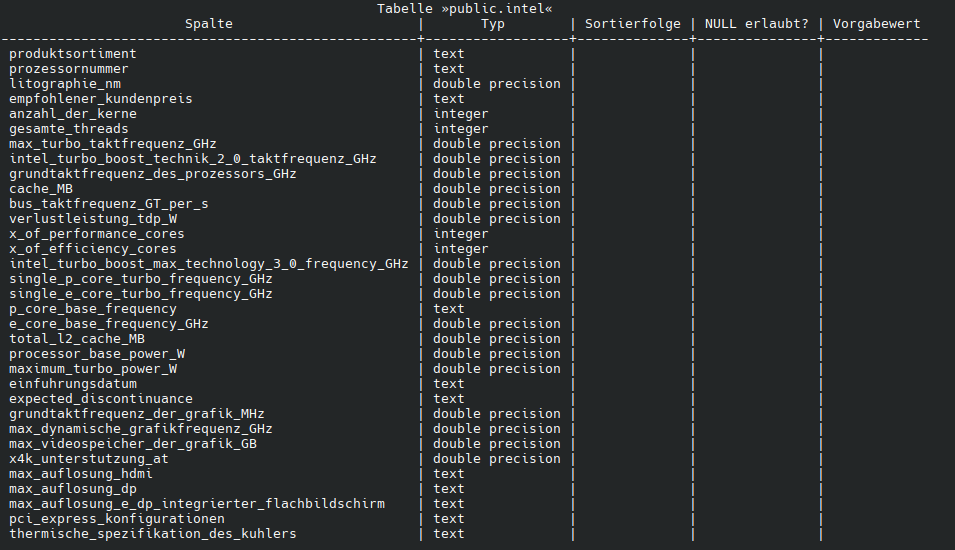
\includegraphics[width=\textwidth]{\imagedir/datenbank_schema.png} 
	\captionsetup{format=hang}
	\caption[Datenbankschema]{\label{fig:datenbankschema}Datenbankschema erstellt durch das R-Skript}
\end{figure}